
\documentclass[journal,12pt,twocolumn]{IEEEtran}
\usepackage{tkz-euclide} % loads TikZ and tkz-base
\usepackage{hyperref}
\usepackage{xcolor}
\title{AI1110 Software Project Report}
\author{Uttam Paharia\\ (CS22BTECH11060)}
\date{\today}

\begin{document}

\maketitle

\section{Introduction}
The Music Player project is a simple application that allows users to play and control the playback of audio files. This project is implemented using the Pygame library in Python, which provides functionality for graphics and audio. The application provides basic functionalities such as playing the next or previous song, pausing and resuming the playback, and displaying the currently playing song.

\section{Implementation}
The project is organized into classes and functions to handle different aspects of the music player. The code is structured as follows:

\begin{itemize}
\item Importing necessary libraries and initializing Pygame.
\item Defining color constants using Pygame's Color class.
\item Creating the Pygame screen and initializing the mixer for audio playback.
\item Defining a Button class to represent the control buttons in the music player.
\item Setting up the initial song list and play stack.
\item Creating instances of the Button class for previous, next, and play buttons.
\item Setting up the main loop to handle events and update the screen.
\item Handling button clicks and updating the play stack accordingly.
\item Loading and playing the selected song using Pygame's mixer.
\end{itemize}

\subsection{Dependencies}
To run the Music Player, the following dependencies are required:

\begin{itemize}
\item Python 
\item Pygame library
\item NumPy library
\end{itemize}

Additionally, the following modules are used:

\begin{itemize}
        \item sys
        \item os
\end{itemize}

\section{Conclusion}
The Music Player project provides a basic music player application with features such as playing audio files, controlling playback, and displaying the currently playing song. It demonstrates the use of Pygame and its audio capabilities in Python programming.

\section{Code}
The code for the Music Player can be found at:\\
\textcolor{blue}{\href{https://github.com/Uttam-Paharia/Probability/tree/main/pythonproject}{\textbf{GitHub link}}}
\begin{figure}[h]
        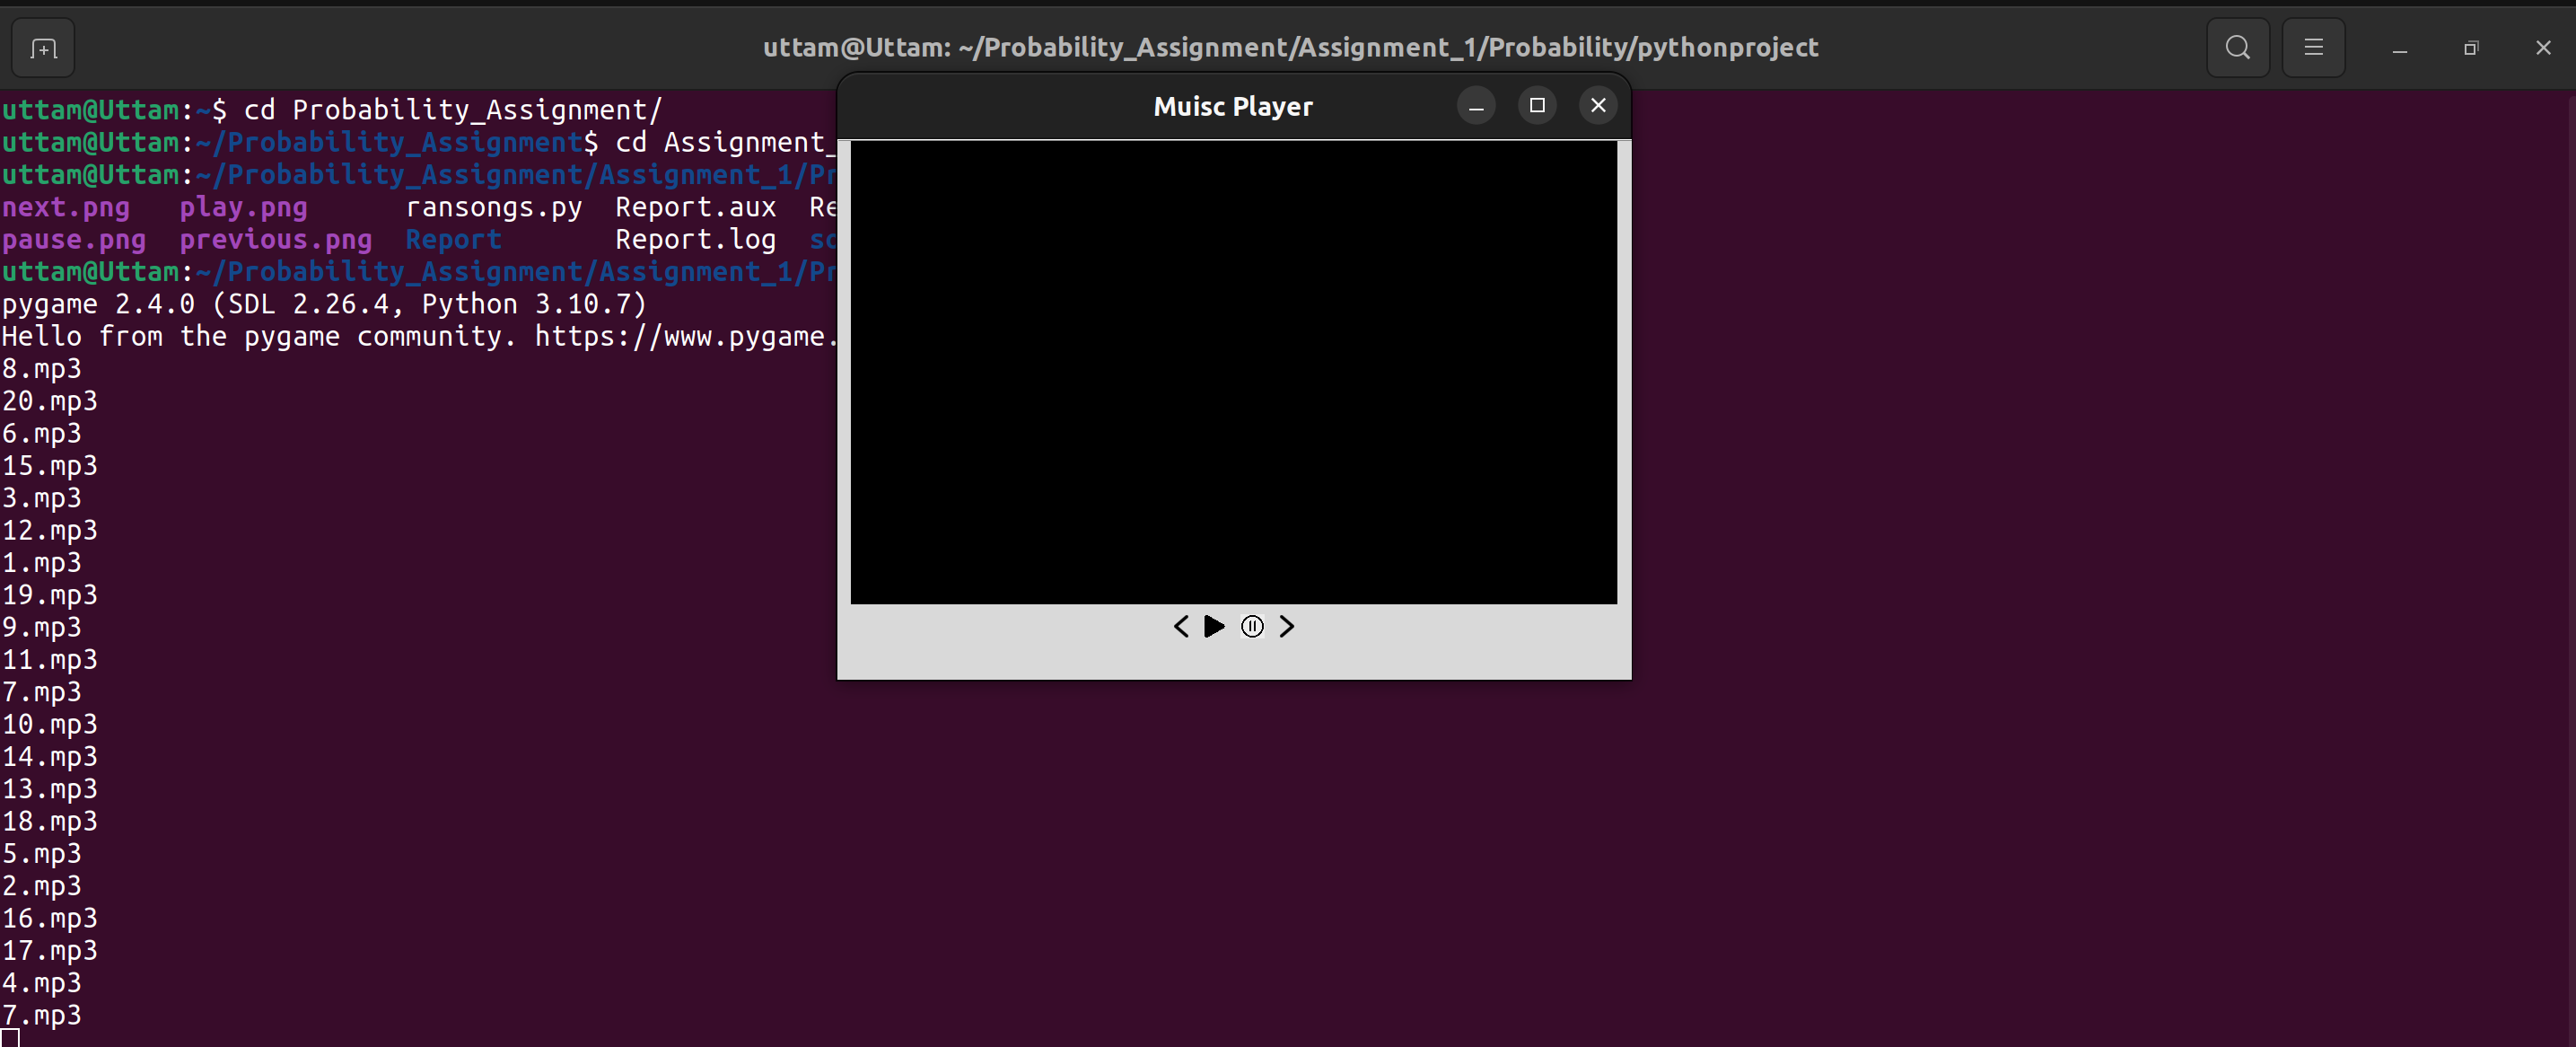
\includegraphics[width=\linewidth]
{project.png}
        \caption{Result}
\end{figure}

\end{document}